\chapter{Part A: Black-Scholes and Monte Carlo pricer}
Developer: Simon Leger

\noindent Validator: Aloke Mukherjee


%DEVELOPER WRITES THIS PART --->

\section{Requirements}

%<description of the problem being solved, relevant equations, algorithms, etc>
In this section, we write a model to price European options using
the Black-Scholes formula and return the greeks associated to
these options. We also write a monte carlo pricer to be able to
check the prices for these options.

The formula for European options is depending on the type of the
options (i.e. Call or Put) is :
$$C(S,T)=S\mathcal{N}(d_1)-Ke^{-rT}\mathcal{N}(d_2)$$
$$P(S,T)=Ke^{-rT}\mathcal{N}(-d_2)-S\mathcal{N}(-d_1)$$
where :
$$d_1=\frac{ln(S/K)+(r+\sigma^2/2)T}{\sigma \sqrt{T}}$$
$$d_2=\frac{ln(S/K)+(r-\sigma^2/2)T}{\sigma \sqrt{T}}$$

and the greeks are :

\begin{center}
\begin{tabular}{|c|c|c|}
\hline
    {\bf } & {\bf Calls} & {\bf Puts} \\
\hline
{\bf delta} &     {$\mathcal{N}(d_1)$} &     {$\mathcal{N}(d_1)-1$} \\
\hline
{\bf gamma} & \multicolumn{ 2}{|c|}{{$\frac{\phi(d_1)}{S\sigma \sqrt(T)}$}} \\
\hline
{\bf vega} & \multicolumn{ 2}{|c|}{${S\phi(d_1)sqrt(T)}$} \\
\hline
{\bf theta} &     {$-\frac{S\phi(d_1)\sigma}{2sqrt(T)}-rKe^{-rT}\mathcal{N}(d_2) $} &     {$-\frac{S\phi(d_1)\sigma}{2sqrt(T)}+rKe^{-rT}\mathcal{N}(-d_2)  $} \\
\hline
 {\bf rho} &     {$KTe^{-rT}\mathcal{N}(d_2)$} &     {$-KTe^{-rT}\mathcal{N}(-d_2)$} \\
\hline
\end{tabular}
\end{center}

We then extend the previous model to provide the same results for
the following strategies :
    - Long Call Spread
    - Long Straddle
    - Long Butterfly Spread

\section{Design }

We have two folders for this part : one named BlackScholes which contains
the BlackScholes class which represents one european option and an OptionStrategy class
which is basically a portfolio of such options and provide important methods for them
as an easy way to create some options inside.


\section{Approach}
%<high-level description of the design>
To construct this, we see two important parts :
\begin{itemize}
    \item One pricer using formula
    \item A generic pricer using Monte Carlo approach
\end{itemize}

One class (named Black-Scholes) computes the prices, implied vol and
greek letters for a given type of option (type is either Call or
Put) and all this should be easily used through a nice
OptionStrategy class which is basically a portfolio of options. In
this class you have the ability to add options by giving their
parameters or use friendly methods that construct for you some
famous combinations, as has been specified in the requirements.

Then we build a multiple-class based monte Carlo pricer which is
driven by the MCEngine class. This pricer should be general enough
to price various derivatives products as it generates a path for
given dates, by taking into account the yield curve and the
volatility surface built in this project, hence the possibility to
price asian, look back options, etc.


\section{Choices}
%<any important design choices you made, e.g. data structures, class hierarchy, algorithm, etc. and a justification for the decision>
\par We did not choose to use polymorphism for the black-Scholes and
option strategy parts as both could be considered independent and
use separately.

\par For the Monte Carlo pricer we used polymorphism in order for the user
to be able to use different random number generators and still have
a robust interface Random class. The default number generator is
Sobol which is better than the default number generator of C++ and
provides enough numbers to be generated if required.

\par In addition, the user has a drift class that can be modified
easily to adopt other path generators. This one uses the extended
Black-Scholes model by taking into account the yield curve and the
volatility surface so they are not considered constant through the
path, which is useful for path dependent options.

\par Then there is a GaussianProcess class which takes the lognormal
process by adding the drift and the random numbers generated and
applying the corresponding volatility.

\par The Payoff class provides methods to take the path generated and
the strike and returns the payoff according to the option
specified.

\par There are four different sorts of number generators : the C++
default generator, the Park Miller generator, the Mersenne Twister
generator and also Sobol which is a quasi random generator. Here is
a comparison of precision for the different number generators : we
try to price a european call, the exact price being 4.94387 :
\bigskip

\begin{tabular}{|r|cc|cc|cc|cc|}
\hline
           & \multicolumn{ 2}{|c|}{300k} & \multicolumn{ 2}{|c|}{1M} & \multicolumn{ 2}{|c|}{10M} & \multicolumn{ 2}{|c|}{50M} \\
\hline
 Generator &      Price &       Time &      Price &       Time &      Price &       Time &      Price &       Time \\

     RandC &       4.96 &      2.156 &      4.935 &      7.172 &     4.9432 &      70.98 &     4.9461 &     355.62 \\

ParkMiller &      4.987 &      1.968 &      4.962 &      6.532 &     4.9448 &       67.7 &     4.9446 &     324.09 \\

MersenneTwister &      4.936 &      1.984 &      4.949 &      6.547 &     4.9461 &      65.08 &     4.9435 &     325.73 \\

     Sobol &    4.94354 &       1.95 &    4.94372 &       6.42 &    4.94385 &      64.26 &    4.94387 &     319.95 \\
\hline
\end{tabular}

\bigskip

As we can see, Sobol is way above the other generators for this kind
of test. Obviously the goal of a monte carlo number generator is to
try to fit at best the interval [0,1] and for this a quasi number
generator is much better than any pseudo generator. The only point
is that the numbers are less random from a general point of view,
since anyone can predict the next number, which is also possible for
any algorithm but usually less easy. For 300,000 paths, we have the
same precision with Sobol, than with Mersenne Twister for 50 million
paths ! And Mersenne Twister is known as the best pseudo random
number generators.  To meet the same precisions as the other pseudo
generators, the C++ random number generator requires 5 times more
paths and it is slower.

\section{Unit tests}

%<short descriptions of each subtest>
The unit test for this part was to build a market environment with a volatility surface and a yield curve and to compute the price of a european call and then to check the price with the monte carlo pricer, after we checked some results with both online pricers and a pricer built in Excel with the closed formula given by the Black-Scholes model.

\section{Performance}

%<how can the performance of this component be sped up by 100%?>
We first implemented this pricer using double* instead of valarray$<$double$>$ and the performance was much better (almost two times faster). This is due to a fixed cost when you read a valarray due to the cast type, but we chose to keep the version with valarray for a better integration with the rest of the code and to make it uniform and easier to read.

Another point could be to test other quasi random number generators
to see if they are more accurate than Sobol, and also to make an
interface for these random number generators to allow a multi
dimensional generation for rainbow options for exemple. The
implementation of Sobol algorithm is done with calibration up to 6
dimensions but we didn't use it since the interface has been done
for one dimension generation.

The last but not least point is that especially in banks, where most
of computers have two processors, it is possible to design the code
so that it can use two threads to take advantage of the available
CPUs.  An easier way that we tested was to create two executable
files and run them on a same machine (dual core Intel processor
2.8Ghz), but in this case one has to be careful about the
initialization of the random number generators otherwise the price
would be the same on the two threads. After this, one just has to
take the average of these prices. This would improve the performance
by 80\%, and maybe up to 250\% with four threads on a machine with
two processors with hyperthreading but we couldn't do this test
since our dual core machine didn't have hyperthreading.

%VALIDATOR WRITES THIS PART --->

\section{Validation}

The closed form formulas for European Calls and Puts as well as the
Greeks Delta and Vega were coded in Matlab (see BS.M in the data
directory).  These were then used to validate the C++ output.  The
Matlab version of Black-Scholes is quite simple to implement since
there already exists functions to calculate the cumulative normal
distribution.

\begin{figure}[htbp]
\begin{center}
        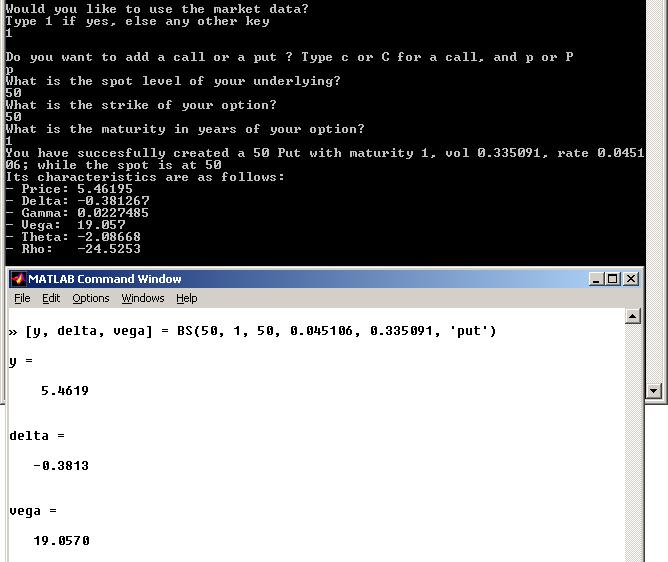
\includegraphics[width=12cm]{blackscholes-matlab.jpg}
        \caption{Verifying Put value with Terreneuve and Matlab}
\end{center}
\end{figure}

Another approach to validation was comparing with the results
obtained by the use of the binomial tree.  Since a binomial tree is
less accurate than the closed forms for European options the value
of this approach is debatable.  Nonetheless it was observed that the
binomial tree results were close to the closed form and Monte Carlo
solutions.

\begin{figure}[htbp]
\begin{center}
        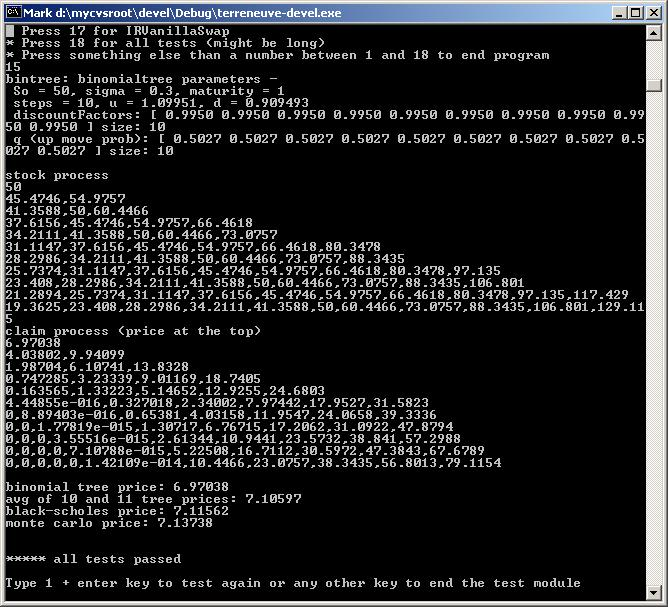
\includegraphics[width=12cm]{blackscholes-bintree.jpg}
        \caption{Comparing Black-Scholes and Monte Carlo Call value with Binomial Tree}
\end{center}
\end{figure}
